

\section{Usage of ANTLR 4}
\label{antlr}
We have based part of our Analyzer on ANTLR 4 parser generator. ANLTR 4 implements Adaptive $LL(*)$ \cite{parr2014adaptive} parsing strategy.

\subsection{Adaptive $LL(*)$ parsing strategy}
Adaptive $LL(*)$ (or short $ALL(*)$) parsing strategy is a combination of simple, efficient and predictable top-down $LL(k)$ parsing strategy with power of $GLR$ which can handle non-deterministic and ambiguous grammars. 
Authors move the grammar analysis to parse-time. This lets $ALL(*)$ handle any non-left-recursive context-free grammar rules and for efficiency it caches analysis results in lookahead DFA.

Theoretical time complexity can be viewed as a possible downside of $ALL(*)$. Parsing of $n$ symbols takes $O(n^4)$ in theory. In practice, however, $ALL(*)$ seems to outperform other parsers by order of magnitude.

Despite the theoretical $O(n^4)$ time complexity, it appears that the $ALL(*)$ behaves linear on most of the code, with no unpredictable performance or large footprint in practice. In order to support this, authors investigate the parse time vs file size for languages \texttt{C}, \texttt{Verilog}, \texttt{Erlang} and \texttt{Lua} files. They found very strong evidence of linearity on all tested languages (see the original paper for details).

\subsection{ANTLR 4 pipeline}

ANTLR 4, similar to any other conventional parser generator, processes the inputted code as follows: (1) breaks down the source string into tokens using \textit{lexer} (2) \textit{parser} build parse trees. 

This pipeline in ANTLR 4 is broken into following classes: 

\begin{description}
	\item[\texttt{CharStream}] represents input code,
	\item[\texttt{Lexer}] breaks the inputted code into tokens,
	\item[\texttt{Token}] token representation that includes important information like token type, position in code or the actual text,
	\item[\texttt{Parser}] builds parse trees,
	\item[\texttt{TokenStream}] connects the lexer and parser.
\end{description}

\cref{antlr_pipeline} sketches the described pipeline.

\begin{figure}[H]
	\centering
	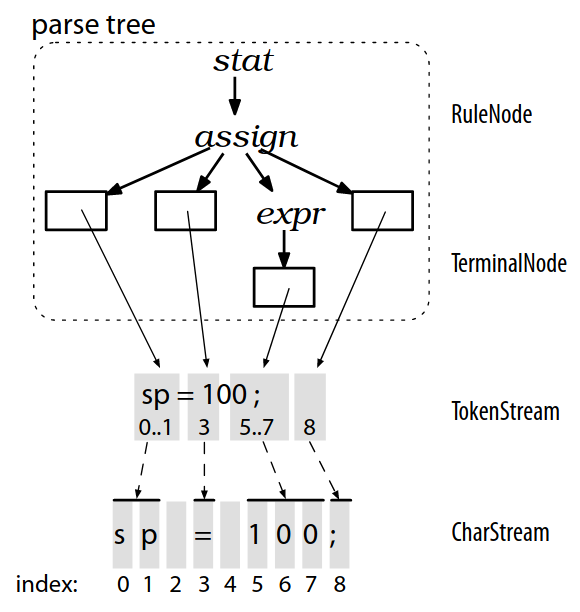
\includegraphics[width=6cm]{img/antlr_pipeline}
	\caption{ANTLR 4 pipeline overview. Taken from \cite{parr2013definitive}.}
	\label{antlr_pipeline}
\end{figure}

\subsection{Parse-Tree walking}

We employ the ANTLR 4 Parse-Tree Visitors during the expression evaluation. ANTLR 4 offers two mechanisms for tree-walking: the parse-tree listeners and parse-tree visitors. As the tree-walker encounters a rule, it triggers a \emph{start} function. Similarly, when the walker visits all children of the node, it calls the \emph{finish} function.  The second mechanism is the parse-tree visitor. The visitor lets the programmer control the walk by explicitly calling methods to visit children. We picked the latter approach because we need to have ampler control over the evaluation (such as operator priority).

\subsection{Visitor}

We employ ANTLR \emph{visitor} feature during evaluation of CA expressions. 

The ANTLR 4 first generates \texttt{hlasmparserVisitor} and \texttt{hlasmparserBaseVisitor}. The former is a abstract class, the latter is a simple implementation of the former. Both classes define ``visit'' functions for every grammar rule. A visit function has exactly one argument --- the context of the rule. The simple implementation executes \texttt{visitChildren()}. Our parse-tree visitor --- the \texttt{expression\_evaluator} --- overrides \texttt{hlasmparserBaseVisitor}. In order to evaluate a sub-rule, we call \texttt{visit(ctx->sub\_rule())}, where \texttt{ctx->sub\_rule()} returns the context of the sub-rule. The \texttt{visit()} function matches appropriate function of the visitor based on the context type (for example, \texttt{visit(ctx->sub\_rule())} would call \texttt{visiSub\_rule(..)}).

\section{Lexer}
\sourceref{parser\_library/include/shared/lexer.h}
Lexer's responsibility is to read source string and break it into tokens --- small pieces of text with special meaning. The most important properties of the lexer:
\begin{itemize}
	\item each token has a location in the source text,
	\item has the ability to check whether all characters are valid in the HLASM source,
	\item can jump in the source file backward and forward if necessary (for implementation of instructions like AGO and AIF). Because of this, it is not possible to use any standard lexing tool, and the lexer has to be implemented from scratch.
\end{itemize}

As previously mentioned, we designed a custom lexer for HLASM. We have a number of reasons to do so. HLASM language is complex. It was first introduced several decades ago, and the language was during this long time subjected to development. Such a long period made the HLASM language complex. Also, it contains some aggressive features, for example, \texttt{AREAD} or \texttt{COPY}, that can alter the source code at parse time.

Conventional lexing tools are most often based on regular expressions. As discussed above, there are several difficulties that one must consider designing lexer for this particular language. A regular expression-based lexer would be too difficult or even impossible to design\footnote{One could match separate characters from the input and let the parser or semantic analysis deal with some of the described problems. This drastic solution would cost performance, as parsers are usually more performance demanding.}.

\subsection{Encodings}
Source code encodings differ for the used libraries. All strings are encoded in \texttt{UTF} as follows:

\begin{description}
	\item[\texttt{UTF-8}] LSP string encoding,
	\item[\texttt{UTF-16}] offsets (positions in source code) in LSP,
	\item[\texttt{UTF-32}] ANTLR 4 source code representation.
\end{description}

\subsection{Architecture}
\sourcerefsu{parser\_library/include/shared/input\_source.h}
{parser\_library/include/shared/token.h}
{parser\_library/include/shared/token\_factory.h}
Beside of the custom lexer, we altered ANTLR's classes \texttt{Token}, \texttt{TokenFactory} and \texttt{ANTLRInputStream}. The reason is to add custom attributes to token that are vital for later stages of the HLASM code analysis (parsing, semantic analyses, etc.). Lexer functionality is implemented in following classes (see \cref{lexer_arch}):

\begin{figure}
	\centering
	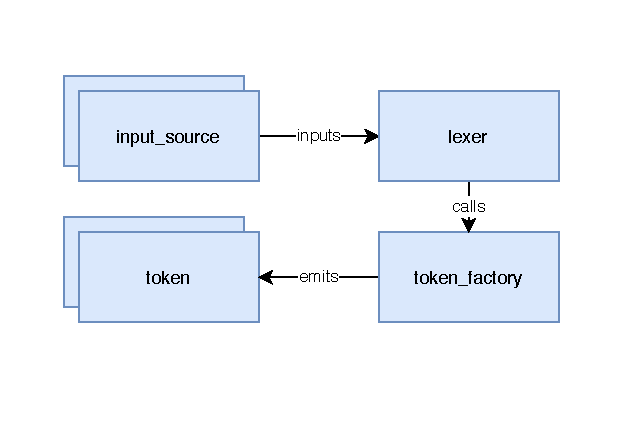
\includegraphics{img/lexer_arch}
	\caption{Lexer architecture overview. Note, there are two \texttt{input\_source}s and there are many \texttt{token}s
		\label{lexer_arch} generated.}
\end{figure}

\begin{description}
	
	\item[\texttt{token}] implements ANTLR's class \texttt{Token} and extends it by adding properties important for location of the token within the input stream. As the LSP protocol works with offsets encoded in \texttt{UTF-16} and ANTLR 4 works with \texttt{UTF-32} encoding, we add attributes for \texttt{UTF-16} positions, too.
	
	Token does not carry the actual text from the source but instead references the position in code (unlike \texttt{CommonToken}). Note that the position of a token is vital for further analysis.
	
	\begin{table}
		\centering
		\begin{tabular}{lr}
			\toprule
			\textbf{IGNORED}                                                                     &  sequence of characters ignored in processing \\
			\textbf{COMMENT}                                                                     &                         commentary statements \\
			\textbf{EOLLN}                                                                       &         token signalling the end of statement \\
			\textbf{SPACE}                                                                       &                          a sequence of spaces \\
			\textbf{IDENTIFIER}                                                                  &                             symbol identifier \\
			\textbf{ORDSYMBOL}                                                                   &                    Ordinary symbol identifier \\
			\textbf{PROCESS}                                                                     &                       process statement token \\
			\textbf{NUM}                                                                         &                                        number \\
			\textbf{ATTR}                                                                        & apostrophe that serves as attribute reference \\
			\thead{\textbf{ASTERISK, SLASH, MINUS, PLUS,}\\ \textbf{LT, GT, EQUALS, LPAR, RPAR}} &                             expression tokens \\
			\thead{\textbf{DOT, COMMA, APOSTROPHE,}\\ \textbf{AMPERSAND, VERTICAL}}              &                        special meaning tokens \\ \bottomrule
		\end{tabular}
		\caption{Enumeration of tokens.}
		\label{tab06:tokens}
	\end{table}
	
	Interesting remark of HLASM language complexity is absence of \emph{string} token (see \cref{tab06:tokens}). Lexer does not generate this token due to existence of model statements (see \cref{var_sym}). There, variable symbol can be written anywhere in the statement (even in the middle of the string), what significantly restricts lexer.
	
	\item[\texttt{token\_factory}] produces tokens of previously described custom type \texttt{token}.
	
	\item[\texttt{input\_source}] implements \texttt{ANTLRInputStream} which encapsulates source code. This implementation adds API for resetting, rewinding and rewriting input. 
	
	Beware of the usage of \texttt{UTF} encodings: \texttt{\_data} (source code string) and positions/indices in API are in \texttt{UTF-32}; \texttt{getText} returns \texttt{UTF-8} string.
	
	\item[\texttt{lexer}] is based on ANTLR's \texttt{TokenSource} class. As most lexers, it is also, in principle, a finite state machine. The most important difference compared to conventional FSMs and other lexers is added communication interface that connects the parser and the instruction interpreter with the lexer. Unusual is also input rewinding (to support \texttt{AREAD}, for example), lexing from parallel sources (\texttt{AINSERT} buffer), and some helper API for subsequent processing stages.
	
	Important functions:
	
	\begin{description}
		\item[\texttt{nextToken()}] implements main functionality: lexes and emits tokens. Before lexing, the function uses the right input stream (either the source code or \texttt{AINSERT} buffer if not empty). After choosing the right input source, the lexer emits token is lexed. HLASM introduces \textit{continuation} symbol (an arbitrary non-blank symbol at column 72 by default) that breaks one logical line into two or more lines in code. The end of one logical line indicates \texttt{EOLLN} token. Such token is important for further (syntactic and semantic) analysis.
		
		
		\item[\texttt{create\_token()}] creates token of given type. The lexer's internal state gives the position of the token. 
		
		\item[\texttt{consume()}] consumes character from the input stream and updates lexer's internal state (used in \texttt{create\_token()}).
		
		\item[\texttt{lex\_tokens()}] lexing of most of the token types.
		
		\item[\texttt{lex\_begin()}] up to certain column, the input can be ignored (can be set in HLASM).
		
		\item[\texttt{lex\_end()}] lexes everything after continuation symbol.
		
		
	\end{description}
	
\end{description}


\section{Parser}
\label{lab06:parser}

Parser component takes the tokens produced by lexer from token stream and recognizes HLASM statements.

\subsection{ANTLR overview}

The input to ANTLR is a grammar written in antlr-specific language that specifies the syntax of HLASM language. The framework takes grammar and generates source code (in C++) for a recognizer, which is able to tell whether input source code is valid or not. Moreover, it is possible to assign a piece of code that executes every time a grammar rule is matched by the recognizer to further process the matched piece of code and produce helper structures (statements).

The parser inherits from the recognizer to provide further operations.

\subsection{Parser workflow}
\sourcerefsu{parser\_library/src/parser\_impl.h}
{parser\_library/src/semantics/range\_provider.h}
Parser (in code referenced as \TT{parser\_impl}) implements opencode statement provider interface. This means that, according to the statement passing in \cref{lab06:proc_stat}, parser needs to parse each statement in \emph{two steps}:

\begin{enumerate}
	\item Parser calls rule \TT{label\_instr}. It parses label and instruction fields into respective structures. The operand and remark field is stored as string.
	\item After retrieving processing format, parser selects corresponding rule to parse operands. With the rule, it parses remaining string from the previous step.
\end{enumerate}

For the means of parsing remaining strings, parser subcomponent contains actually \emph{two parsers}. The first one parses statement after statement from a source file. The second parses the operands from the string passed by the first parser. 

Operands to have correctly set ranges prior to the source file rather than to the passed string, parser uses \emph{Range provider}. It helps the second parser to have ranges of reparsed operands consistent with the ranges of other fields. It is initialized with the begin location of operand field in the statement and all ranges furtherly created in parsing are adjusted to have correct boundaries.

\subsection{Statement structure}
\sourcerefsu{parser\_library/src/semantics/collector.h}
{parser\_library/src/semantics/statement.h}
{parser\_library/src/semantics/statement\_fields.h}
During parsing of a statement, several structures are created and collected. They are \TT{label\_si, instruction\_si, operand\_si, remark\_si} (\emph{si} as semantic information). They are collected with \TT{collector} and built into \TT{statement\_si} structure.

Label and instruction structures can contain either identifier of a symbol or --- when in model statement --- concatenation of strings and variable symbols. Remark field is simply just a string as it serves as a commentary statement field. Operand field contains list of operands used in the statement. They can be of several formats.

\subsubsection{Concatenation}
\sourcerefsu{parser\_library/src/semantics/concatenation.h}
A model statement is a statement that contains variable symbol in any of the statement fields. This variable symbol is further to be substituted by an arbitrary string and then re-parsed. Hence, the field is represented by a concatenation of helper structures. The concatenation can be further evaluated to produce the final string.

The helper structures are:
\begin{itemize}
	\item \TT{char\_str} -- character string.
	\item \TT{var\_sym} -- substitutable variable symbol.
	\item \TT{dot}, \TT{equals} -- characters with special meaning.
	\item \TT{sublist} -- by parenthesis enclosed recursive concatenation.
\end{itemize}

\subsubsection{Operand formats}
\sourcerefsu{parser\_library/src/semantics/operand.h}
The statement processor can request parser to retrieve statements with this operand formats:
\begin{itemize}
	\item \emph{machine/assembler/conditional assembly/macro} -- instruction operands. Each type of instruction has it's specific format.
	\item \emph{model} -- operands for model statements. It is a chain of strings and variable symbols.
	\item \emph{deferred} -- operands with not yet known format. Stored as a string.
\end{itemize}

Each operand format has corresponding \emph{operand structure}. They all inherit abstract \TT{operand} and each have various children for different kinds of the operand format (see \cref{fig06:operand_arch}). Assembler and Machine operand structures inherit from \emph{Evaluable operand}. It is a common structure for operand objects that are composed of resolvable objects (see \cref{symbol_dependency_tables}).

\begin{figure}
	\centering
	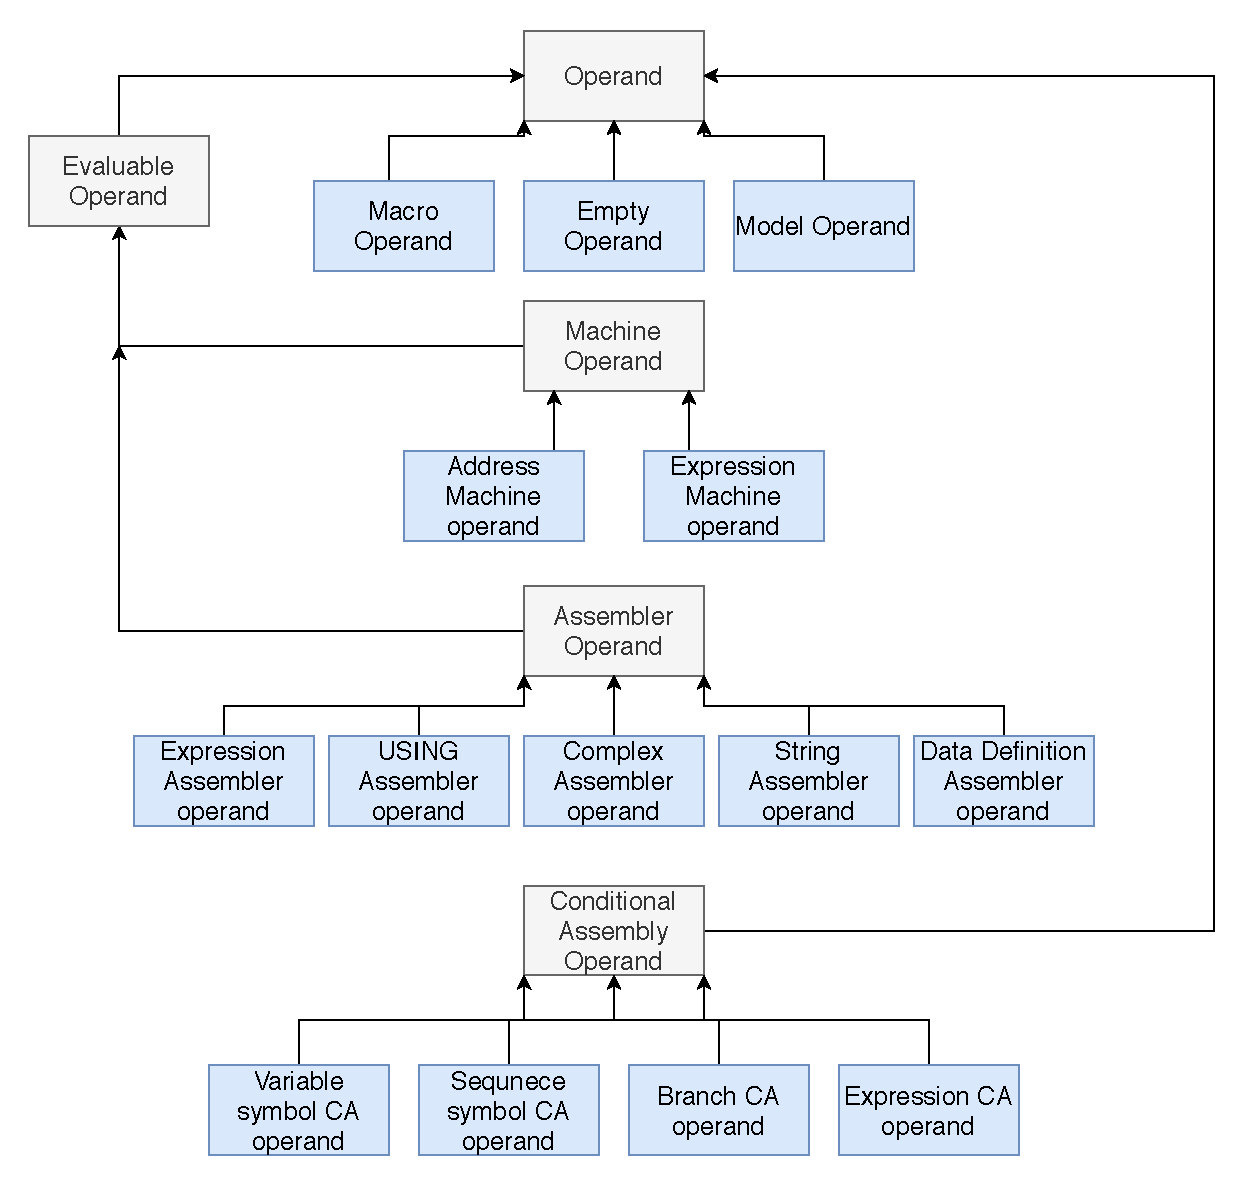
\includegraphics[width=\textwidth]{img/operand_arch}
	\caption{Operand structure inheritance.}
	\label{fig06:operand_arch}
\end{figure}

\subsection{Grammar rules}
\sourcerefsu{parser\_library/src/grammar}
Grammar rules describing parser are separated into several files (see \cref{parser_rules}):
\begin{itemize}
	\item \TT{hlasm\_parser.g4} -- Top level rules are stored here.
	\item \TT{lookahead\_rules.g4} -- Rules for lookahead mode.
	\item \TT{label\_field\_rules.g4} -- Rules taking care of label field of statement.
	\item \TT{instruction\_field\_rules.g4} -- Rules taking care of instruction field of statement.
	\item \TT{operand\_field\_rules.g4} -- Rules taking care of operand field of statement.
	\item \TT{macro/machine/assembler/ca/model/deferred\_operand\_rules.g4} -- Concrete operand field rules.
	\item \TT{ca/asm\_expression\_rules.g4} -- Rules for expressions.
	\item \TT{data\_def\_rules.g4} -- Rules for data definition.
\end{itemize}

